\documentclass[12pt,a4paper]{article}

\usepackage[left=3cm, right=3cm, top=2.5cm, bottom=2.5cm, headheight=38.40865pt]{geometry} % Adjusted headheight
\usepackage{setspace}
\usepackage{amsmath}
\usepackage{tikz}
\usepackage{pgfplotstable}
\usepackage{titlesec}
\usepackage{bm}
\usepackage{tcolorbox}
\tcbuselibrary{skins}
\usepackage{empheq}
\usepackage{booktabs}
\usepackage{caption}
\usepackage{hyperref}
\usepackage{fancyhdr}
\usepackage{float}
\hypersetup{
    colorlinks=true,
    linkcolor=black,
    filecolor=magenta,      
    urlcolor=cyan,
    pdfpagemode=FullScreen,
    }
\usepackage{graphicx}
\graphicspath{ {./images/} }

\pgfplotsset{compat=1.18}

\titleformat{\section}{\Large\bfseries}{\thesection}{1em}{}
\titleformat{\subsection}{\large\bfseries}{\thesubsection}{1em}{}

\renewcommand{\contentsname}{Table des Matières}
\renewcommand{\tablename}{Tableau}

\title{Force de Laplace}
\author{Liviu Arsenescu, Cătălin Bozan}
\date{23.04.2024}

\newtcbox{\mymath}[1][]{%
    nobeforeafter,
    tcbox raise base,
    enhanced,
    colframe=black,
    colback=white,
    boxrule=1pt,
    drop shadow={
        xshift=3pt, % Removed 'shadow' prefix
        yshift=-3pt, % Removed 'shadow' prefix
        opacity=1
    },
    #1
}

\pagestyle{fancy}
\fancyhf{}
\rhead{
\includegraphics[width=4cm]{hearclogo.png}}
\lhead{\thepage}
\setlength{\headsep}{30pt}

\begin{document}
    \pagenumbering{gobble}
    \begin{titlepage}
        \begin{center}
            \vspace*{\fill}
            \Huge \textbf{Force de Laplace} \\
            \Huge \textbf{Étude du champ magnétique} \\
            \Large Rapport du Laboratoire \\
            \begin{figure}[h]
                \centering
                
\includegraphics[width=7cm]{hearclogo.png}
            \end{figure}
            \vspace{\fill}
            \Large Liviu Arsenescu, Cătălin Bozan \\
            23.04.2024

            \vspace*{\fill}
        \end{center}
    \end{titlepage}

    \thispagestyle{empty}
    \tableofcontents
    \newpage

    \pagenumbering{arabic}
    \section{Description de l'expérience}
    \subsection{Buts}
    \begin{itemize}
        \item Étude de la force de Laplace
        \item Démontrer la dépendance linéaire de la force par rapport au champ magnétique $\bm{B}$
    \end{itemize}

    \subsection{Éléments théoriques}
    \subsubsection{Les différentes grandeurs physiques rencontrées}
    \begin{minipage}{0.6\linewidth}
        \begin{itemize}
            \item $\bm{F_L}$ - force de Laplace
            \item $\bm{P}$ et $\bm{N}$ - force du poids et force normale
            \item $\bm{I}$ - courant électrique
            \item $\bm{l}$ - longueur du conducteur
            \item $\bm{\theta}$ - l'angle entre les vecteurs $I \vec{l}$ et $\vec{B}$
            \item $\bm{m}$ - différentes masses
            \item $\bm{g}$ - l'accélération gravitationnelle de la Terre
        \end{itemize}
    \end{minipage}%
    \hfill
    \begin{minipage}{0.4\linewidth}
        \begin{itemize}
            \item[-] $\bm{[ceva]=unitate}$
        \end{itemize}   
    \end{minipage}

    \subsubsection{Modèle Théoriques}
    Pour décrire le modèle mathématique dont on a besoin, on partira de la formule suivante : 
    \begin{empheq}[box={\mymath}]{equation*}
        \vec{F_L} = I \vec{l} \times \vec{B}
    \end{empheq}
    Comme on le sait, la norme d'un vecteur résultant d'un produit vectoriel peut être écrit comme suit :
    \begin{equation*}
        ||\vec{F_L}|| = ||I \vec{l}|| \cdot ||\vec{B}|| sin(\theta) \Rightarrow ||\vec{F_L}|| = IlBsin{\theta} 
    \end{equation*}

    Pour la configuration de la bobine, on peut représenter les forces agissant comme suit :
    \begin{figure}[H]
        \centering
        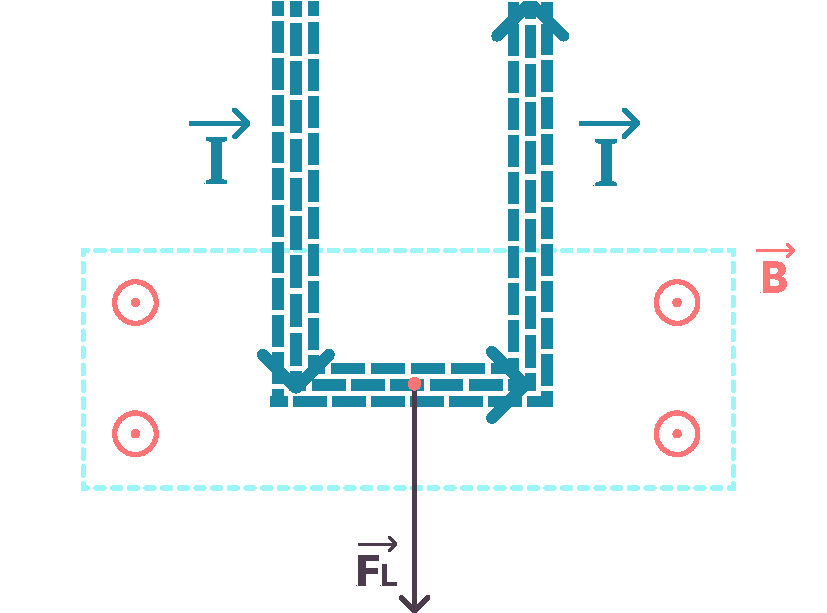
\includegraphics[scale=0.5]{images/magnet_coil.pdf}
        \caption{Système de forces de la bobine}
    \end{figure}
    En utilisant la troisième loi de Newton, on peut construire le système de forces suivant sur l'aimant :
    \begin{figure}[H]
        \centering
        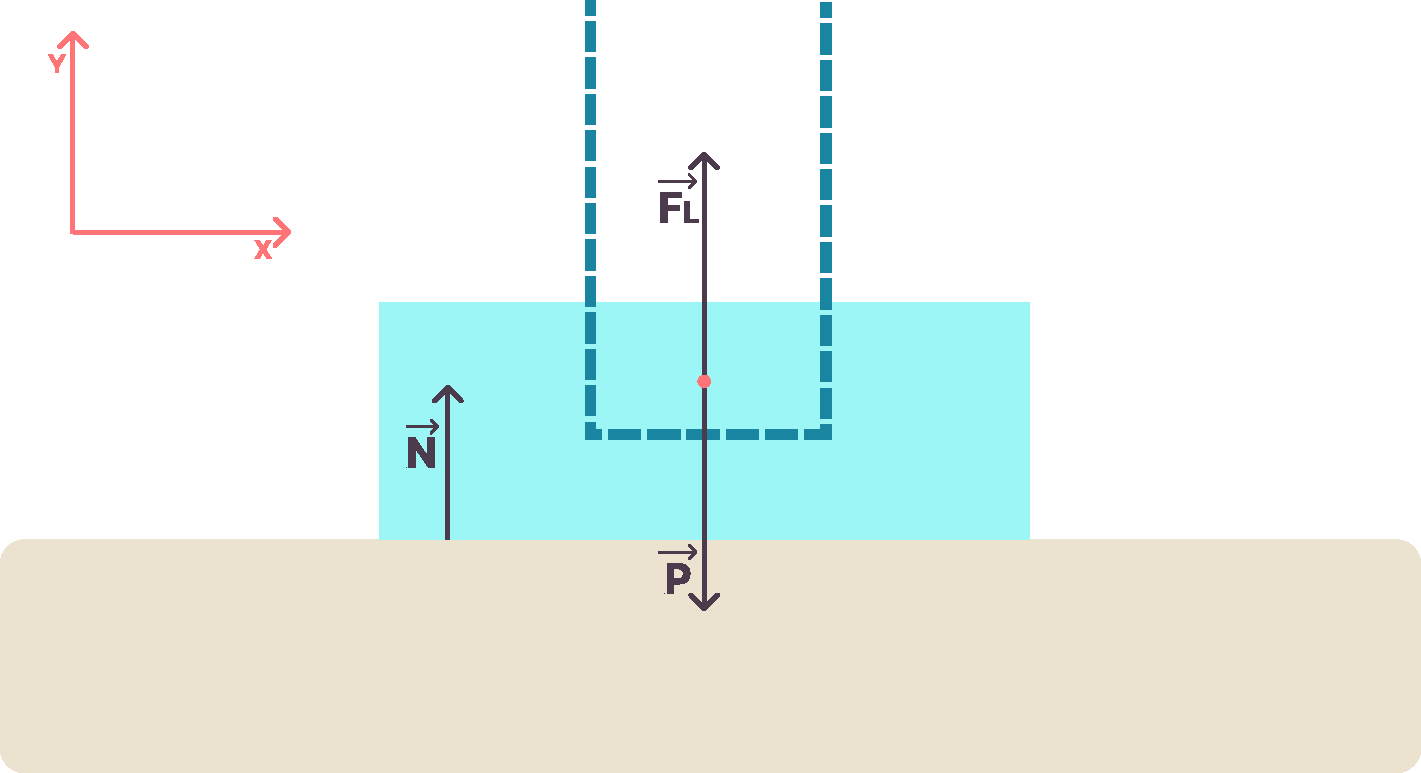
\includegraphics[scale=0.5]{images/magnet_side.pdf}
        \caption{Système de forces sur l'aimant}
    \end{figure}
    En utilisant la deuxième loi de Newton dans la dernière figure, on obtient :
    \begin{equation*}
        \Sigma \vec{F} = 0 \Rightarrow \vec{F_L} + \vec{N} + \vec{P} = 0
    \end{equation*}
    On observe que les forces agissent uniquement sur l'axe y, ce qui permet de déduire l'équation suivante :
    \begin{equation*}
        \pm F_L + N - P = 0
    \end{equation*}
    En alimentant la bobine en courant, on constate que deux masses différentes apparaissent sur la balance :
    \begin{itemize}
        \item $m_0$ - masse de l'aimant
        \item $m_1$ - masse apparente de l'aimant
    \end{itemize}
    Avec ces deux mesures, on peut développer à nouveau l'équation :
    \begin{align*}
        \pm F_L + m_1g - m_0g &= 0 \\
        |F_L| &= |m_1 - m_0|g \\
        |F_L| &= \delta m g
    \end{align*}
    Où $\delta m$ est le module de la différence entre $m_1$ et $m_0$. \\
    Égalant ce que on a obtenu pour $||\vec{F_L}||$ et pour $|F_L|$, on obtien :
    \begin{equation*}
        \left.
        \begin{aligned}
            |F_L| &= \delta mg \\
            ||\vec{F_L}|| &= IlB\sin(\theta)
        \end{aligned}
        \right\}
        \Rightarrow
        \delta mg = \frac{IlBsin(\theta)}{g}
    \end{equation*}

    \subsection{Principe de l'expérience}
    \subsection{Schéma et montage de l’expérience}
    \subsection{Déroulement de l'expérience}
    \section{Mesures}
    \section{Analyse des mesures et résultats}
    \subsection{Choix et calcul d'incertitudes}
    \subsubsection{Choix des incertitude :}
    \subsubsection{Calcul d'incertitudes}
    \subsection{Discussion des résultats :}
    \section{Synthèse et conclusion}
\end{document}
